\clearpage
\part{Zoe: Inspectable Measurement and Memory}
\label{part:zoe}

\section{Architecture and the epistemic firewall}
Zoe is a native graphical environment for creative geometry, forecast inspection, Bayesian evidence, and replayable memory. It unifies HELEN's lightweight geometry and stored predictions, Ablation's Spatial IR and VDI evidence environment, Cerotto's forensic workbench, brain-gem's chambered notebook, and a deterministic BRAIN observation/recommendation layer. The components share inspection workflows without silently merging their evidence stores or permissions.

The architectural invariant is
\begin{center}
\boxed{\text{measurement}\;\neq\;\text{evidence}\;\neq\;\text{belief update}\;\neq\;\text{action}.}
\end{center}
A stochastic chamber can produce a forecast and a deterministic chamber can measure it. Preserving an observation does not change a posterior. Only an explicit evidence event updates belief. In the original proof of concept, recommendations and Cognitive Field proposals remain review-required with \texttt{executed=False}. That flag describes the execution-path state of the record, not the absence of computation.

\begin{figure}[htbp]
\centering
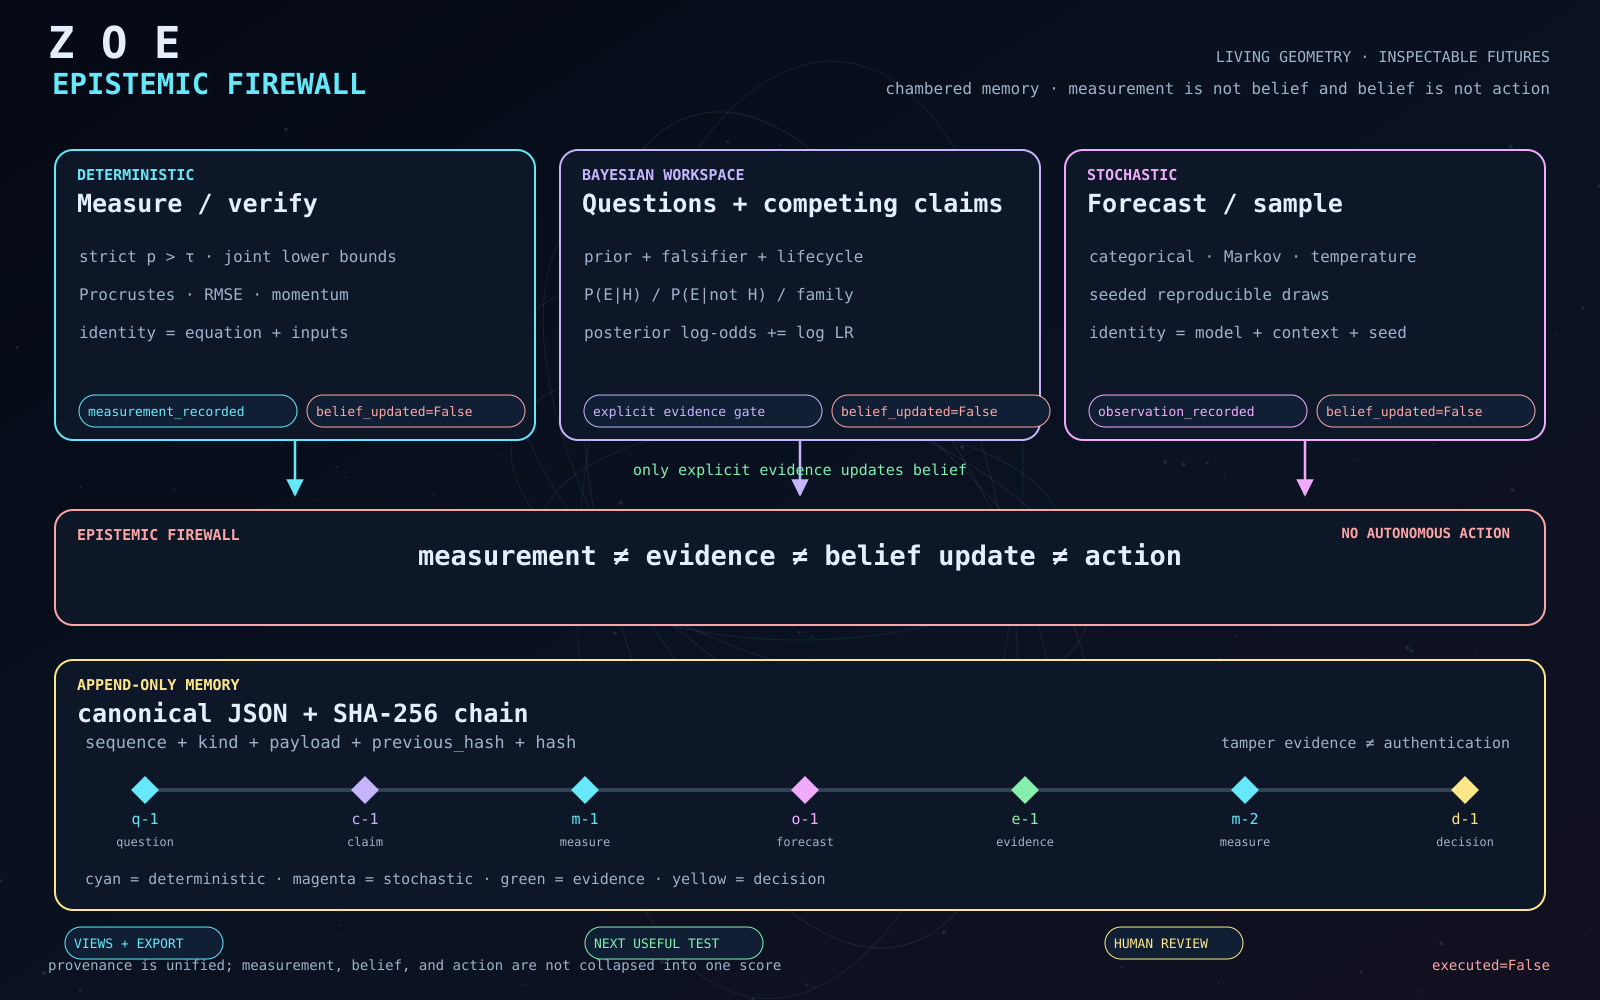
\includegraphics[width=\textwidth]{epistemic-firewall.png}
\caption{The Zoe epistemic firewall. The later self-governing extension changes execution authority only inside a separately declared in-memory loop; it does not erase these epistemic distinctions.}
\label{fig:firewall}
\end{figure}

The native components have distinct scopes:
\begin{itemize}
  \item \textbf{HELEN} supplies lazy scenes, direct interaction, accessible-volume controls, and compressed held-out categorical predictions.
  \item \textbf{Ablation + GEM} supplies native GTK hosting, Spatial IR, Lab sessions, VDI replay, source constraints, and evidence export.
  \item \textbf{Cerotto GEM} supplies read-only forensic cases, guarded evidence actions, vault timelines, and a separate C11 engine and permission model. Zoe does not absorb its database or authority.
  \item \textbf{BRAIN and the field notebook} supply observation state, deterministic recommendations, Bayesian claims and evidence, deterministic/stochastic chambers, and next-test ranking.
  \item \textbf{Cognitive Field and Presence} supply bounded symbolic proposals, state reflection, and an explicitly bounded self-model.
  \item \textbf{PALA} is an optional recovery companion for signature carving and filesystem recovery. Recovered content is not thereby authentic, complete, or safe.
\end{itemize}

\section{Bayesian field notebook}
Questions contain independent binary claims with priors, current posteriors, falsifiers, and lifecycle states. Claims are not forced into a mutually exclusive set. For prior $p$ and supplied likelihoods $L_T=P(E\mid H)$ and $L_F=P(E\mid\neg H)$, an explicit evidence event updates
\begin{equation}
\operatorname{logit}(p')=\operatorname{logit}(p)+\log\frac{L_T}{L_F},
\qquad
\operatorname{logit}(p)=\log\frac{p}{1-p}.
\label{eq:bayes-logit}
\end{equation}
Equivalently, the likelihood ratio is added in log-odds space. Every update preserves the evidence source, likelihood ratio, log likelihood ratio, prior and posterior log-odds, previous and new posterior, and belief diff. Negative and mixed evidence remain in the history.

Posteriors are conditional on the supplied likelihood model, not objective truth scores. Evidence families prevent derivative or correlated sources from silently becoming independent confirmation. Repeating a family requires explicit dependence acknowledgment and adjusted likelihoods. This is a software guard for disciplined bookkeeping, not an automatic estimator of the correct dependence model.

Next-test prioritization uses the declared heuristic
\begin{equation}
\operatorname{priority}(q)=\frac{v_q\,g_q}{\varepsilon_q},
\label{eq:priority}
\end{equation}
where $v_q$ is decision value, $g_q$ expected information gain, and $\varepsilon_q>0$ estimated effort. In the original notebook this ranks attention only: it is not a probability, learned reward, discovered utility, or authorization rule. The later autonomy loop reuses the same arithmetic as an internal proposal utility, a change in control semantics that must be stated rather than hidden.

\begin{figure}[htbp]
\centering
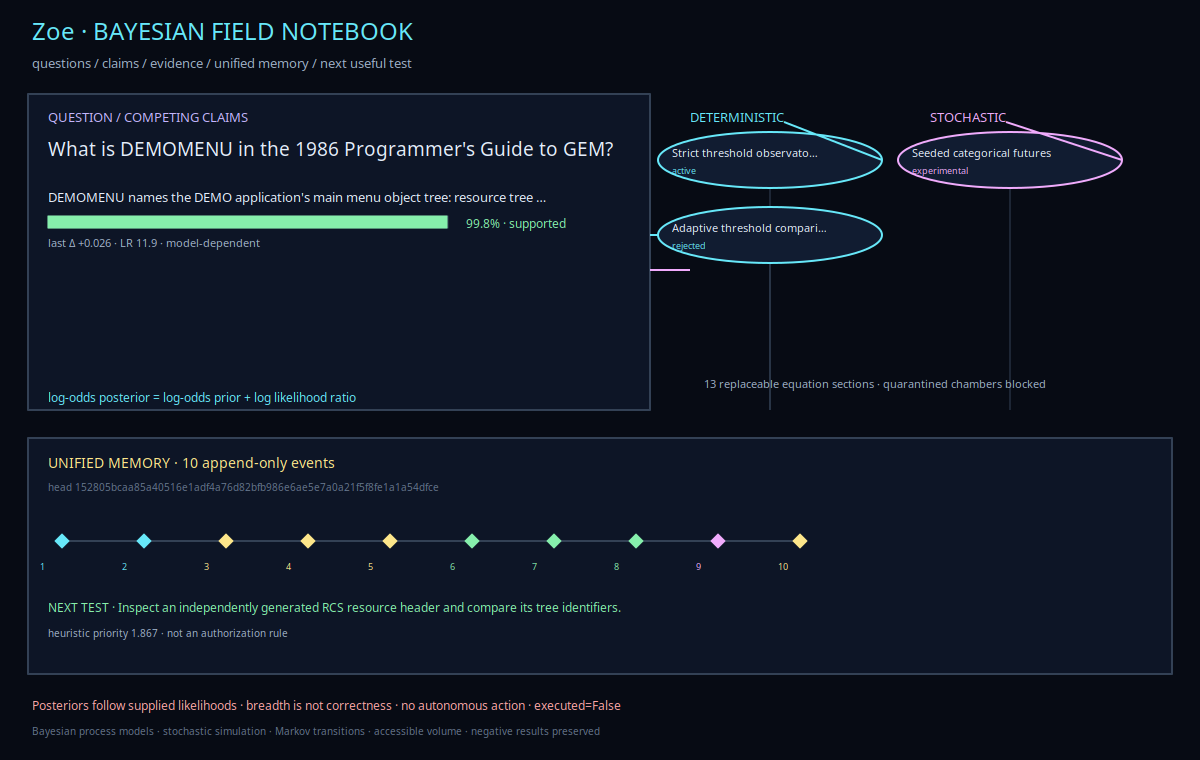
\includegraphics[width=\textwidth]{field-notebook.png}
\caption{Zoe's Bayesian field notebook: explicit evidence updates, deterministic and stochastic chambers, append-only memory, and review-required next-test recommendations.}
\label{fig:notebook}
\end{figure}

The worked DEMOMENU example investigates a definition in the 1986 \emph{Programmer's Guide to GEM}. It retains a primary-source definition, version-dependent counterevidence, initialization-code observations, a strict measurement, a seeded stochastic chamber, and a next-test recommendation. Its value is the inspectable belief history rather than the posterior percentage alone.

\section{Chambers and replayable memory}
The equation registry contains 13 replaceable sections: binary Bayesian updates, strict volume, forecast measurement, adaptive volume, joint volume, momentum, temperature, categorical sampling, Markov steps, bounded continuations, timing RMSE, Procrustes alignment, and inspection priority. Custom functions are registered through a Python API without \texttt{eval}. Deterministic chambers record reproducible measurements; stochastic chambers record forecasts, transitions, transforms, and seeded samples. Quarantined chambers remain inspectable but cannot run.

For sequence $s_i$, event kind $k_i$, payload $p_i$, and previous hash $h_{i-1}$, the canonical chain is
\begin{equation}
h_i=\sha\!\left(\canonical(s_i,k_i,p_i,h_{i-1})\right).
\label{eq:memory-chain}
\end{equation}
Loading recomputes the complete chain and rejects edited or reordered events. Probability vectors of at most 64 values are stored completely; longer vectors are represented by length and SHA-256 digest to bound memory. No-overwrite saves protect earlier exports.

\begin{figure}[htbp]
\centering
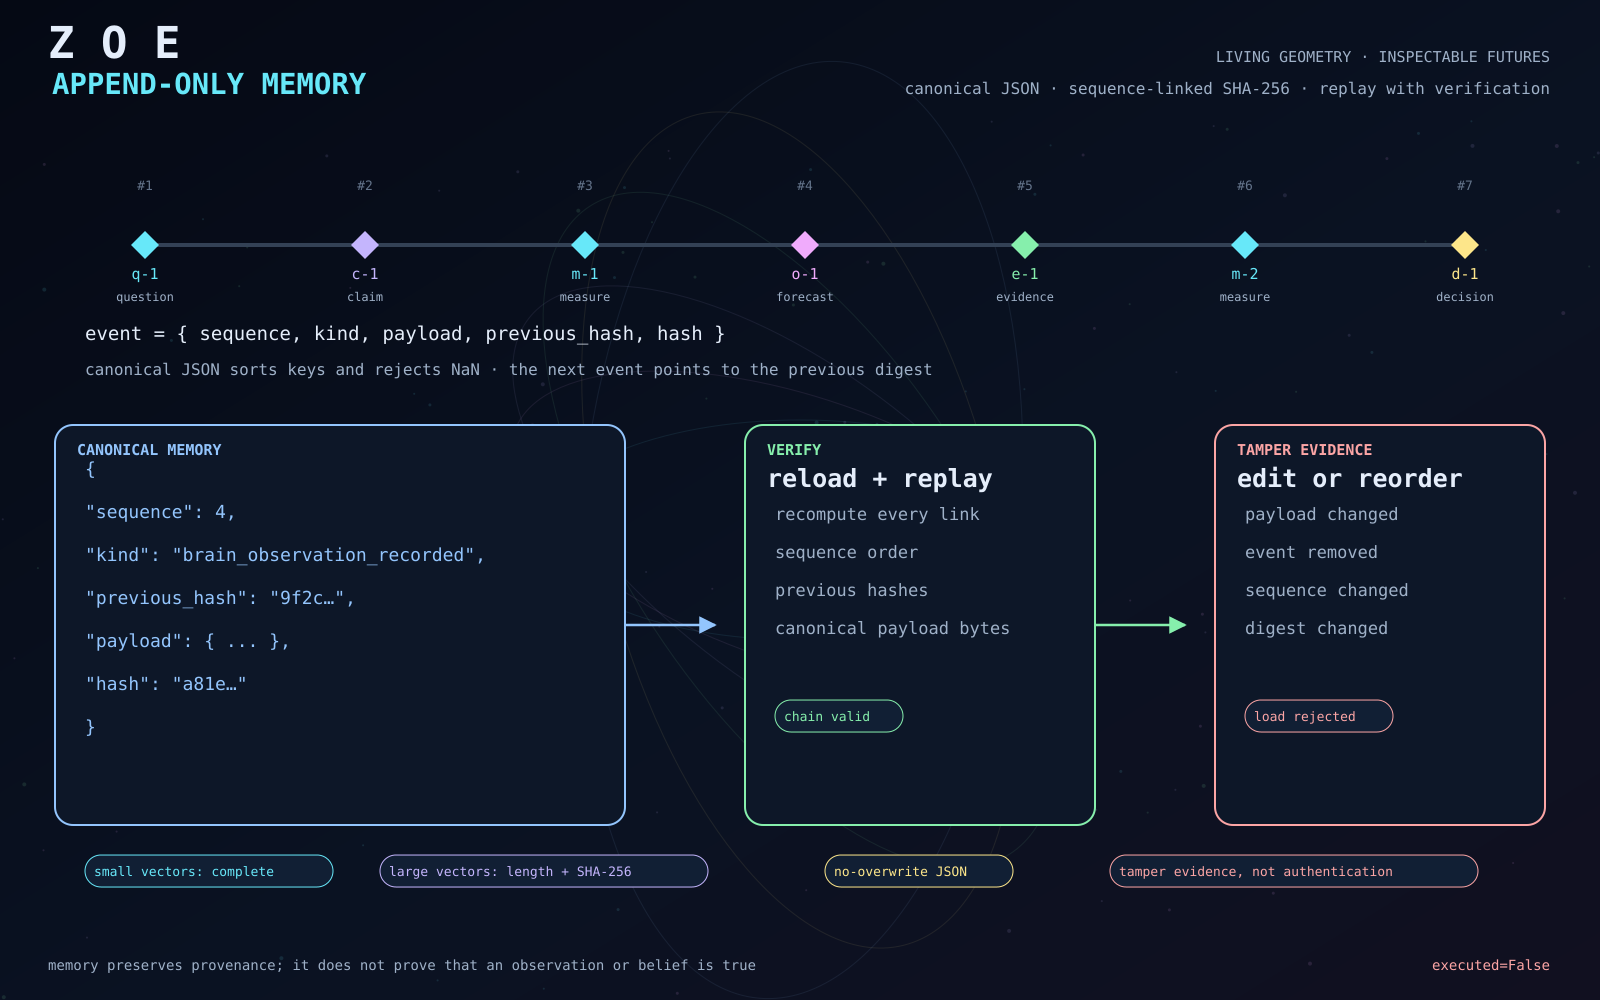
\includegraphics[width=\textwidth]{memory-chain.png}
\caption{Append-only Zoe memory records distinct event kinds and makes alteration visible. Hash chaining supplies tamper evidence, not authentication or proof that a recorded claim is true.}
\label{fig:memory}
\end{figure}

The integrated knowledge graph applies the same canonical-event discipline to repository observations and declared links. A source observation records repository, revision, and scope; a declared link does not transfer evidence or permission. Source presence is not runtime verification. These distinctions are central when multiple independently governed components appear in one interface.

\section{Cog: a bounded categorical token processor}
Zoe Cog is a deliberately small trainable bigram processor, not an LLM. For context token $u$, let $n_u(a)$ be the observed count of candidate $a$, $N_u=\sum_an_u(a)$, and $q(a)$ the unigram prior. With smoothing $\alpha\in(0,10]$,
\begin{equation}
\widetilde p(a\mid u)=\frac{n_u(a)+\alpha q(a)}{N_u+\alpha},
\qquad
p(a\mid u)=\frac{\widetilde p(a\mid u)}{\sum_{b\in\mathcal O}\widetilde p(b\mid u)}.
\label{eq:cog-bigram}
\end{equation}
Backward walks apply the same construction to reversed transition counts and reverse unigram counts. Each walk selects maximum probability with lexical tie-breaking and measures the complete distribution using the unchanged strict operator. Reversing a transition relation does not reverse meaning, causality, or time.

Cog exposes forward and backward walks, complete probabilities, source hashes, volume bands, and experimental temperature steering. Generated walks are review-required and do not assert facts or authorize commands. The small vocabulary makes the processor suitable for deterministic counterfactual experiments in the autonomy study, but token interventions are not distributions over feasible real-world actions.

\section{Cognitive Field, BRAIN, and Presence}
\subsection{Bounded symbolic proposal generation}
The Cognitive Field implements a bounded General Symbol Processor, where ``general'' refers to explicit text, tags, record IDs, revisions, and human-readable rule descriptions rather than unrestricted intelligence. Sourced inputs enter a bounded FIFO working set. Declarative storage and retrieval check revisions. A procedural rule $r$ with required tag set $T_r$ matches working-set tags $T_W$ when
\begin{equation}
\operatorname{Match}(r,W)=\indicator[T_r\subseteq T_W].
\label{eq:cognitive-match}
\end{equation}
Rules contain no executable code. A successful match can prepare a proposal, but in the original Zoe build it remains \texttt{review\_required=True}, \texttt{belief\_updated=False}, and \texttt{executed=False}. The worked example uses capacity four, records an eviction, preserves a revision mismatch, and shows that only one of two declared rules matches. This is symbolic software behavior, not a validated model of biological memory, ACT-R, Spaun, or consciousness.

\begin{figure}[htbp]
\centering
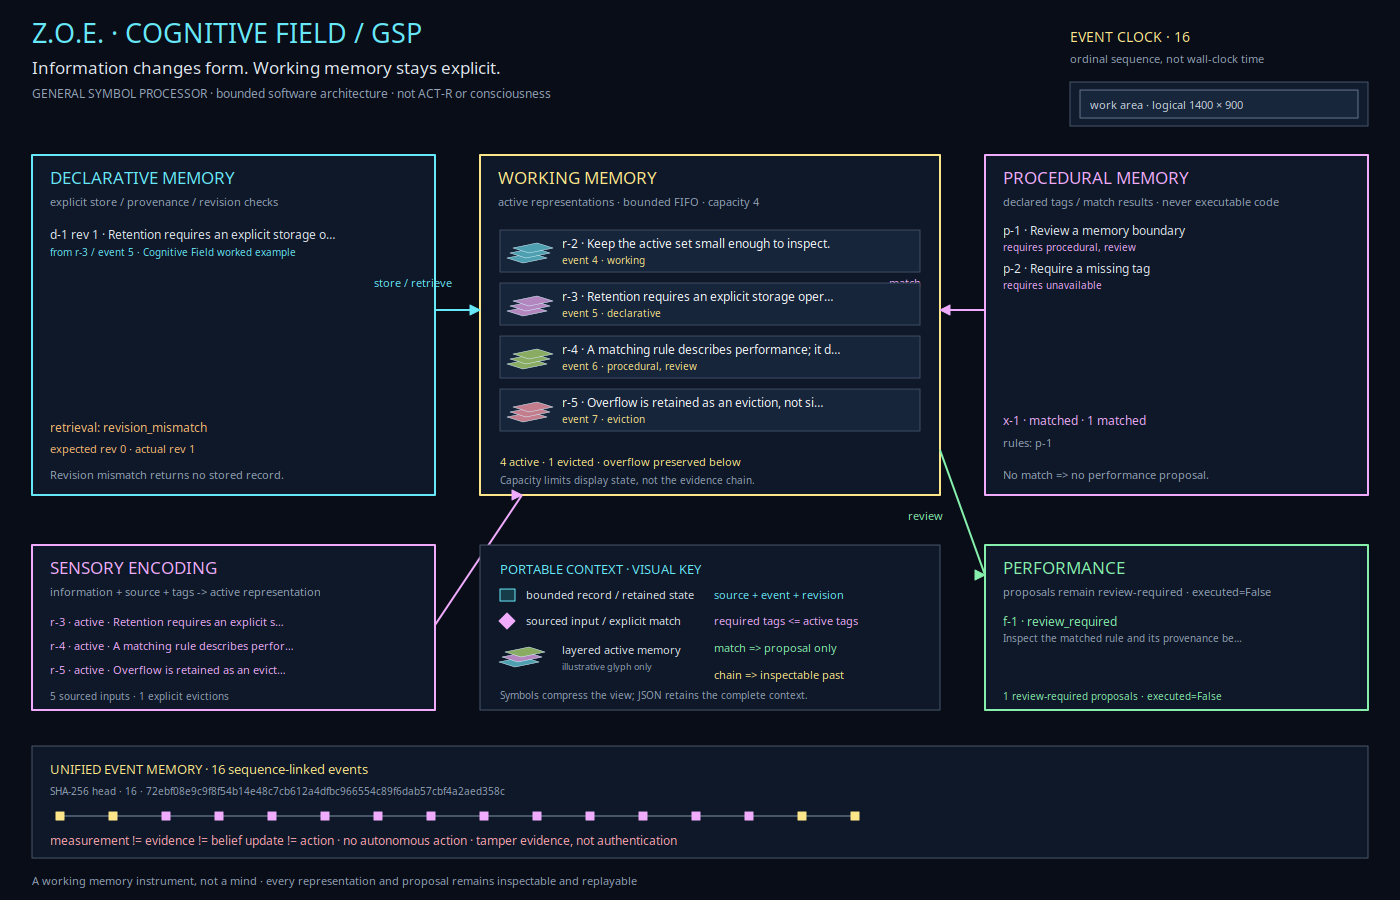
\includegraphics[width=\textwidth]{cognitive-field.png}
\caption{Zoe's Cognitive Field: sourced bounded working memory, declarative revision checks, procedural matching, and review-required proposals.}
\label{fig:cognitive}
\end{figure}

\subsection{Deterministic observation and recommendation}
BRAIN records forecast and evidence state and returns a deterministic module/action recommendation. In schematic form,
\begin{equation}
o_t=M_{\mathrm{BRAIN}}(S_t,C_t),\qquad
r_t=R_{\mathrm{BRAIN}}(o_t),
\label{eq:brain}
\end{equation}
where $r_t$ is advice, not execution. The autonomy benchmark exercises four states: an in-band correct forecast, a broad out-of-band forecast, an incorrect forecast, and an in-band correct forecast after evidence export. They yield four distinct recommendations: \texttt{research/preserve}, \texttt{volume/inspect}, \texttt{research/inspect}, and \texttt{horizon/inspect}. This variation supplies the state-responsiveness dimension later denoted $R$.

\subsection{Self-model boundary}
Presence preserves reflections, uncertainty, provenance, and a self-model while explicitly recording that a self-model is not a self. Self-reports can be evidence about the system's generated representation; they are not self-certification of experience, correctness, or autonomy. Presence does not turn a high accessible-volume count or a proposal into phenomenal perception.

\begin{figure}[htbp]
\centering
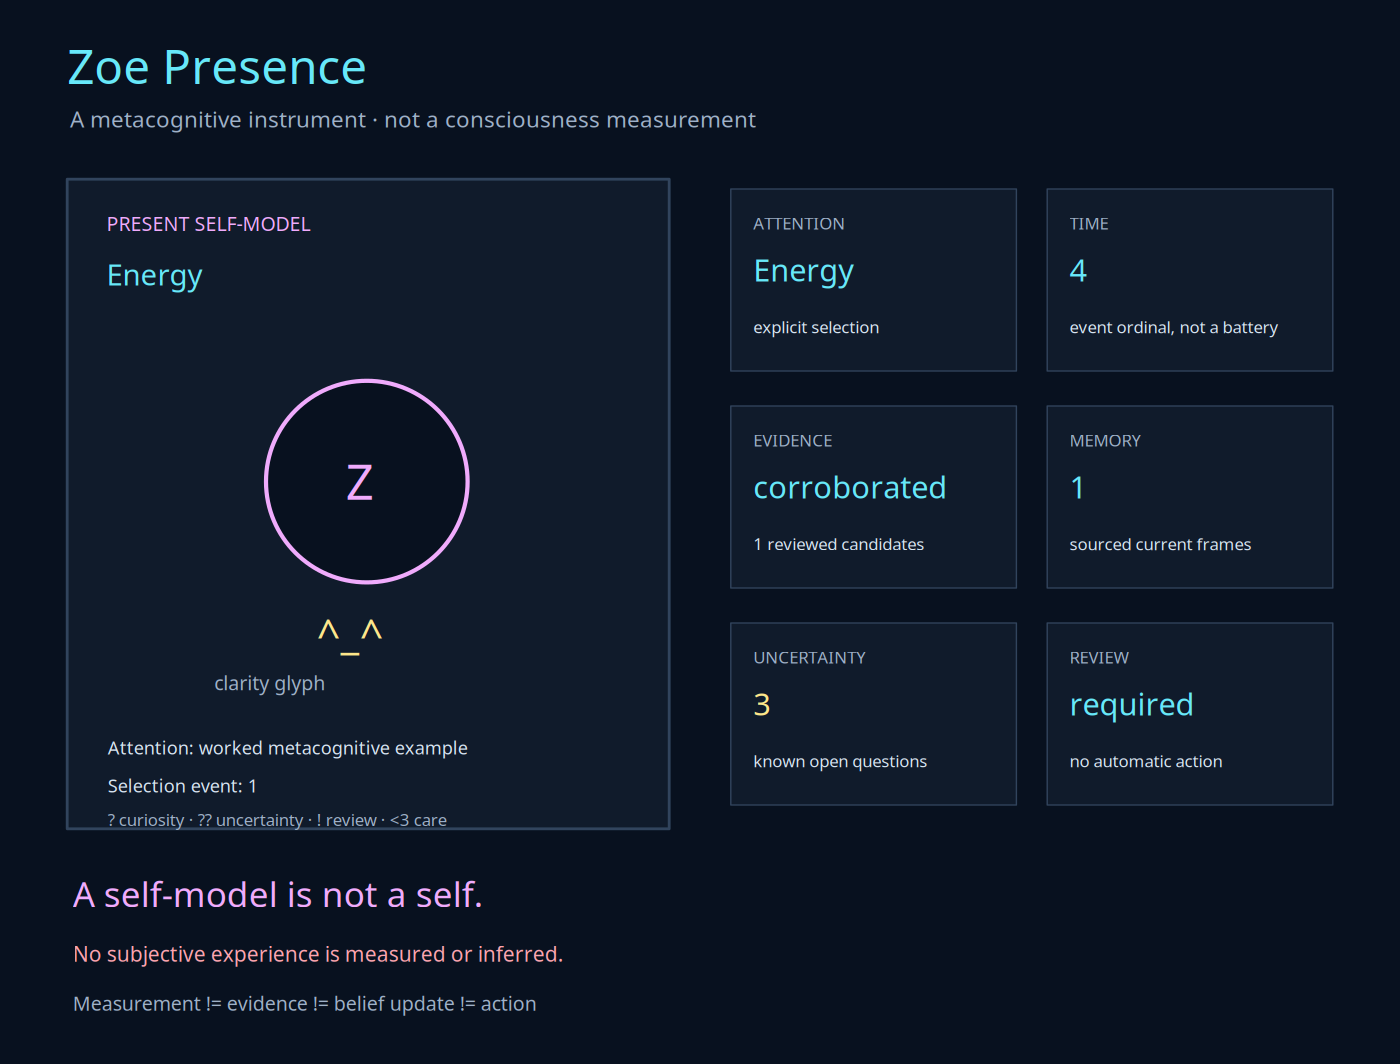
\includegraphics[width=\textwidth]{presence.png}
\caption{Presence exposes a bounded self-model and review boundary without treating self-description as proof of a self.}
\label{fig:presence}
\end{figure}

\section{Native geometry and evidence export}
The native Geometry Atlas supplies similarity, rigid, and affine Procrustes alignment, ellipse families, parabolic envelopes, modular clocks, hub-and-loop graph invariants, accessible-volume controls, and an Onset Lab. Spatial IR scenes can be exported to SVG, PNG, and real little-endian GEM VDI. Headless export does not require GTK. Source-constraint and VDI-roundtrip checks concern deterministic geometry and file behavior, not whole-shape, anatomical, or semantic correctness.

The integrated environment also connects ten source repositories through twelve launch or inspection endpoints in the historical allgems distribution. Each component retains its dependencies, evidence stores, and guards. A plan label cannot prove physical behavior, and a unified interface is not a universal enforcement mechanism.

\section{CERN evidence and virtual workbenches}
\subsection{Inventory, provenance, and process ownership}
The CERN Workbench connects the read-only CERN and Digital Research evidence collections to Zoe-owned process lifecycle controls, HELIOS, and Atelier \cite{zoecernworkbench}. Its handover records 9,968 CERN inventory entries and 226 document previews. The Evidence Navigator's schema-v2 index divides those previews into C1 foundational (40), C2 subsystem (49), C3 integrated (125), and C4 cross-domain (12). Full verification checks 226 source hashes, 226 preview hashes, 226 compatibility links, and 17 bridge-document links. A preview is navigation evidence, not a complete explanation or live detector state \cite{zoevidenceguide}.

The console bridge attaches to a healthy existing loopback server or starts a new one on a free port. It records process ownership and stops only a process it started whose command still matches the expected checkout; it does not terminate an attached user-owned server. Browser opening, XTEST input, and serial emission require explicit actions. Corpus inspection starts no process and accesses no physical hardware.

\begin{figure}[htbp]
\centering
\begin{tabular}{@{}c@{}c@{}}
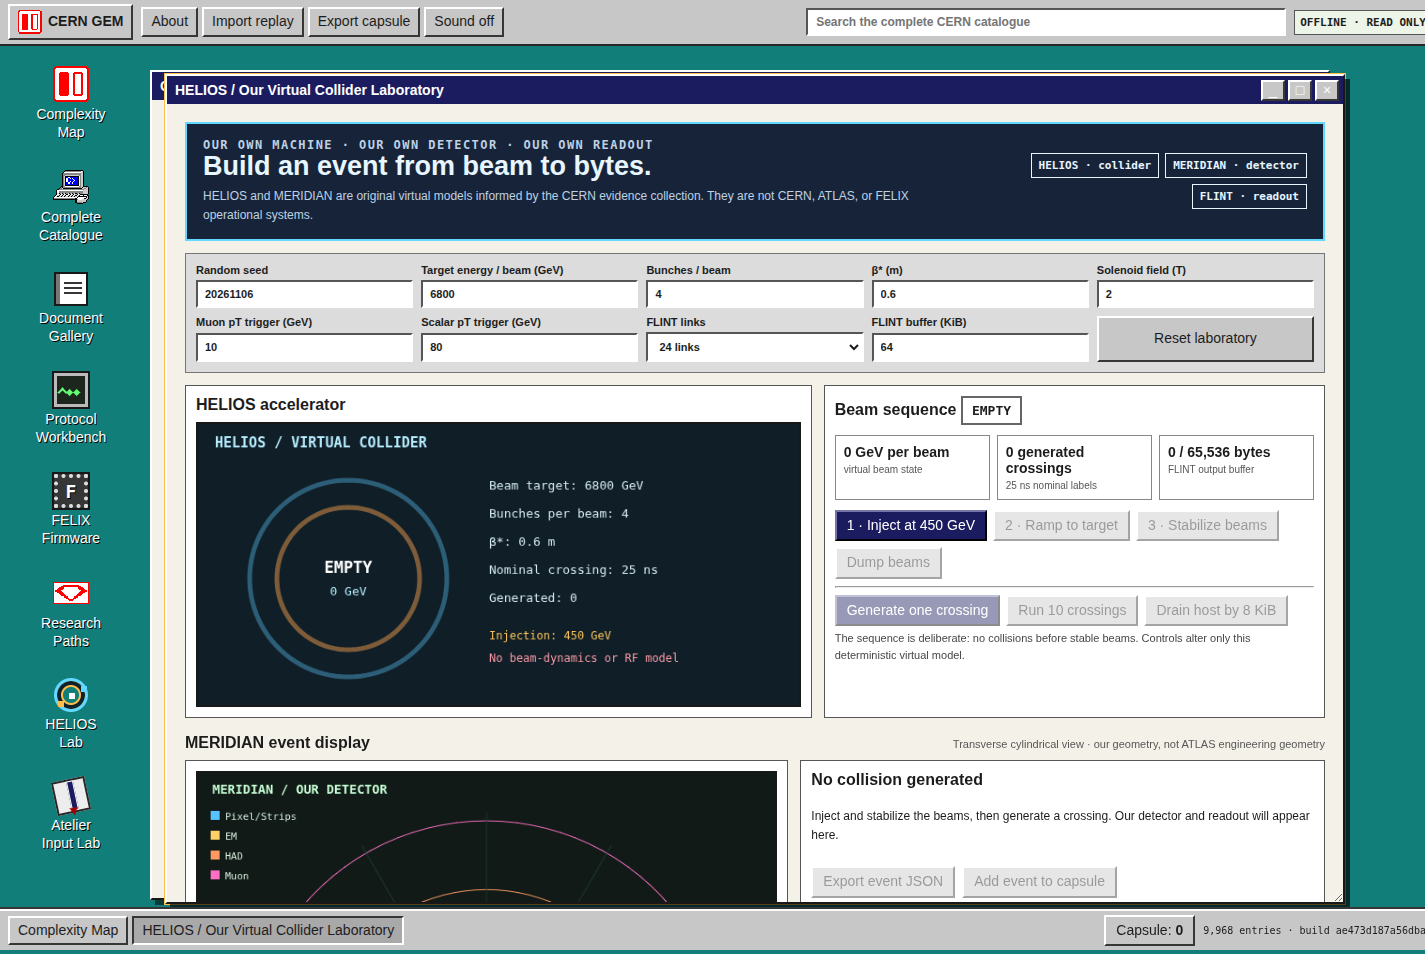
\includegraphics[width=0.48\textwidth]{zoe-helios.png}&
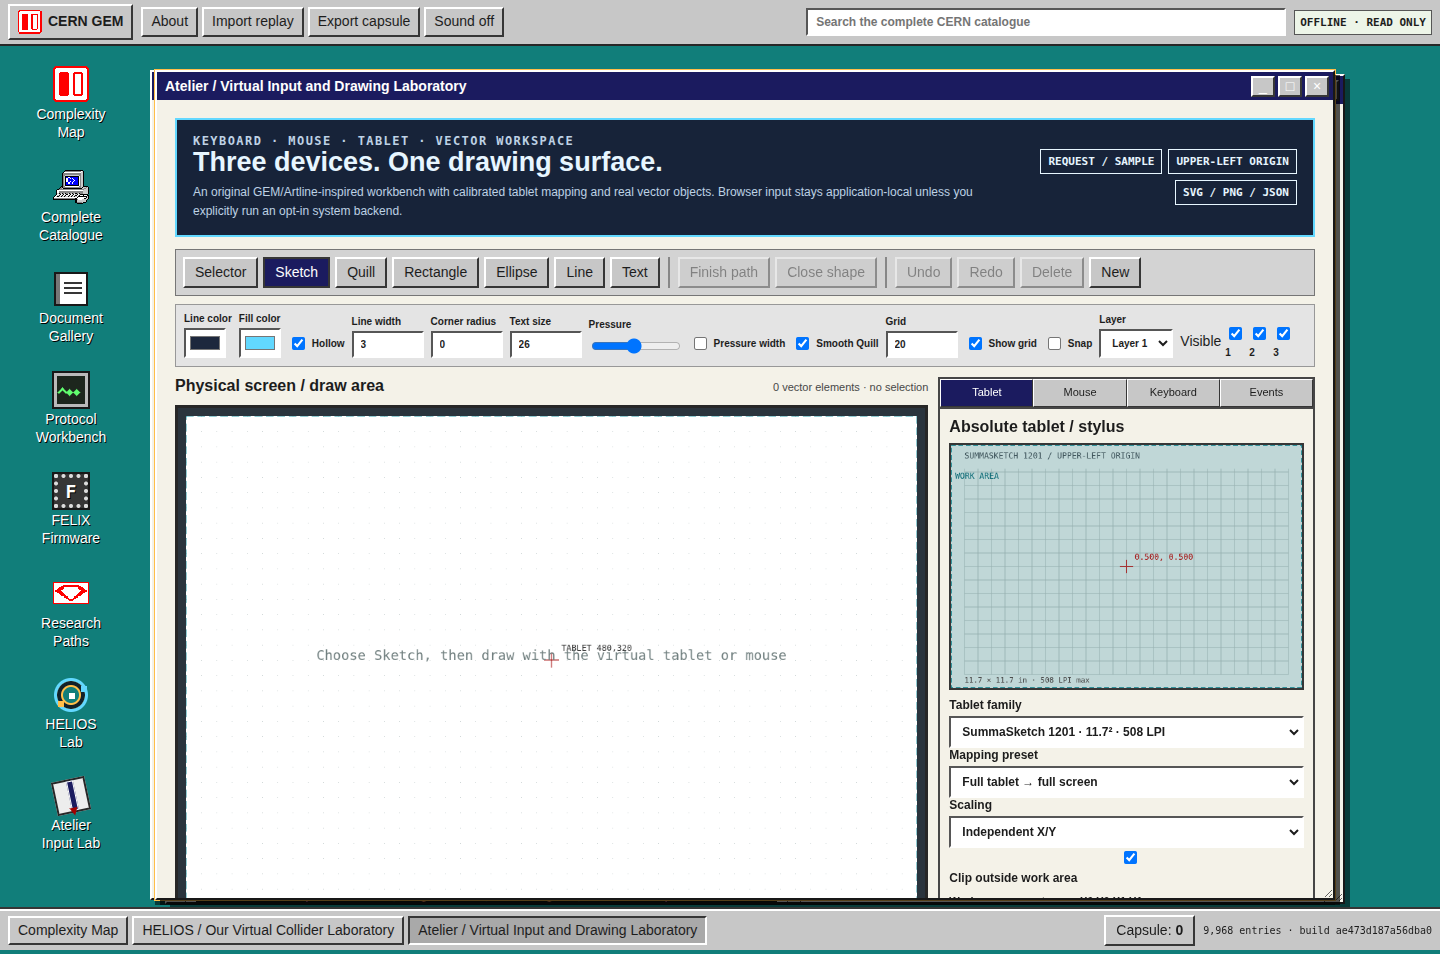
\includegraphics[width=0.48\textwidth]{zoe-atelier.png}
\end{tabular}
\caption{HELIOS and Atelier are virtual collider, input, drawing, and replay laboratories. Their scenes and input models do not imply a physical accelerator connection.}
\label{fig:cern-virtual-labs}
\end{figure}

The historical handover recorded 39/39 Zoe stress tests, 20/20 GEM stress tests, 5/5 CERN corpus tests, 75 Python tests, three JavaScript model suites, and 130 browser checks passing, including isolated live tests only when explicitly enabled. These are scoped implementation checks, not hardware validation.

\subsection{Seven evidence bridges and synthetic timing}
The Evidence Navigator implements seven bridges: timing-aware readout replay, a protocol observation ladder, guarded observability, scene/audio sonification, deterministic shadow retrieval, cross-experiment design review, and C1--C4 practice. Its default timing replay uses 24 channels, 64 events, a 40.08 MHz reference, an eight-slot buffer, 256-byte descriptors, and host consumption every third event. CRC32 protects descriptor integrity but is not a signature. Outputs retain \texttt{hardware\_accessed=false}, \texttt{measured=false}, and \texttt{physical\_connection\_claimed=false}.

The same replay can generate deterministic 16-bit mono PCM audio. Sonification is another view of the recorded synthetic state, not detector sound, an alarm, or a health signal. A shadow query returns saved finding fields without an LLM; a negative static timing result is not automatically a deployed runtime failure.

\subsection{Protocol Lab: recovered framing without device commands}
The Protocol Lab independently implements documented SPECS and AMAC examples \cite{zoeprotocolguide}. The SPECS first header byte is
\begin{equation}
H_0=(\operatorname{slave\ address}\ll2)\,|\,\operatorname{mode}.
\end{equation}
For header bytes $H_0,H_1,H_2$ and check byte $H_3$, the demonstrated nibble check is
\begin{equation}
C=\left(\bigoplus_{i=0}^{2}((H_i\gg4)\oplus(H_i\,\&\,0x0F))\right)\oplus(H_3\gg4),
\qquad H_3\,\&\,0x0F=C.
\end{equation}
Payload bytes are XOR-checked and sent least-significant-bit first; a ninth marker bit identifies the final payload byte. These checks provide integrity information, not authentication.

The recovered short/long boundary is
\begin{equation}
\operatorname{long}=\indicator[\operatorname{read\ count}>0x80],
\qquad \operatorname{reported\ count}=\operatorname{read\ count}\,\&\,0x7F.
\end{equation}
Thus 128 is not long and reports zero, while 129 is long and reports one. Focused RTL evidence covers all 256 counts and 1,280 checks. AMAC read-next independently increments a three-bit sequence and eight-bit address with wraparound; returned data values are supplied separately. The laboratory regenerates models and recorded examples without issuing device commands.

\begin{figure}[htbp]
\centering
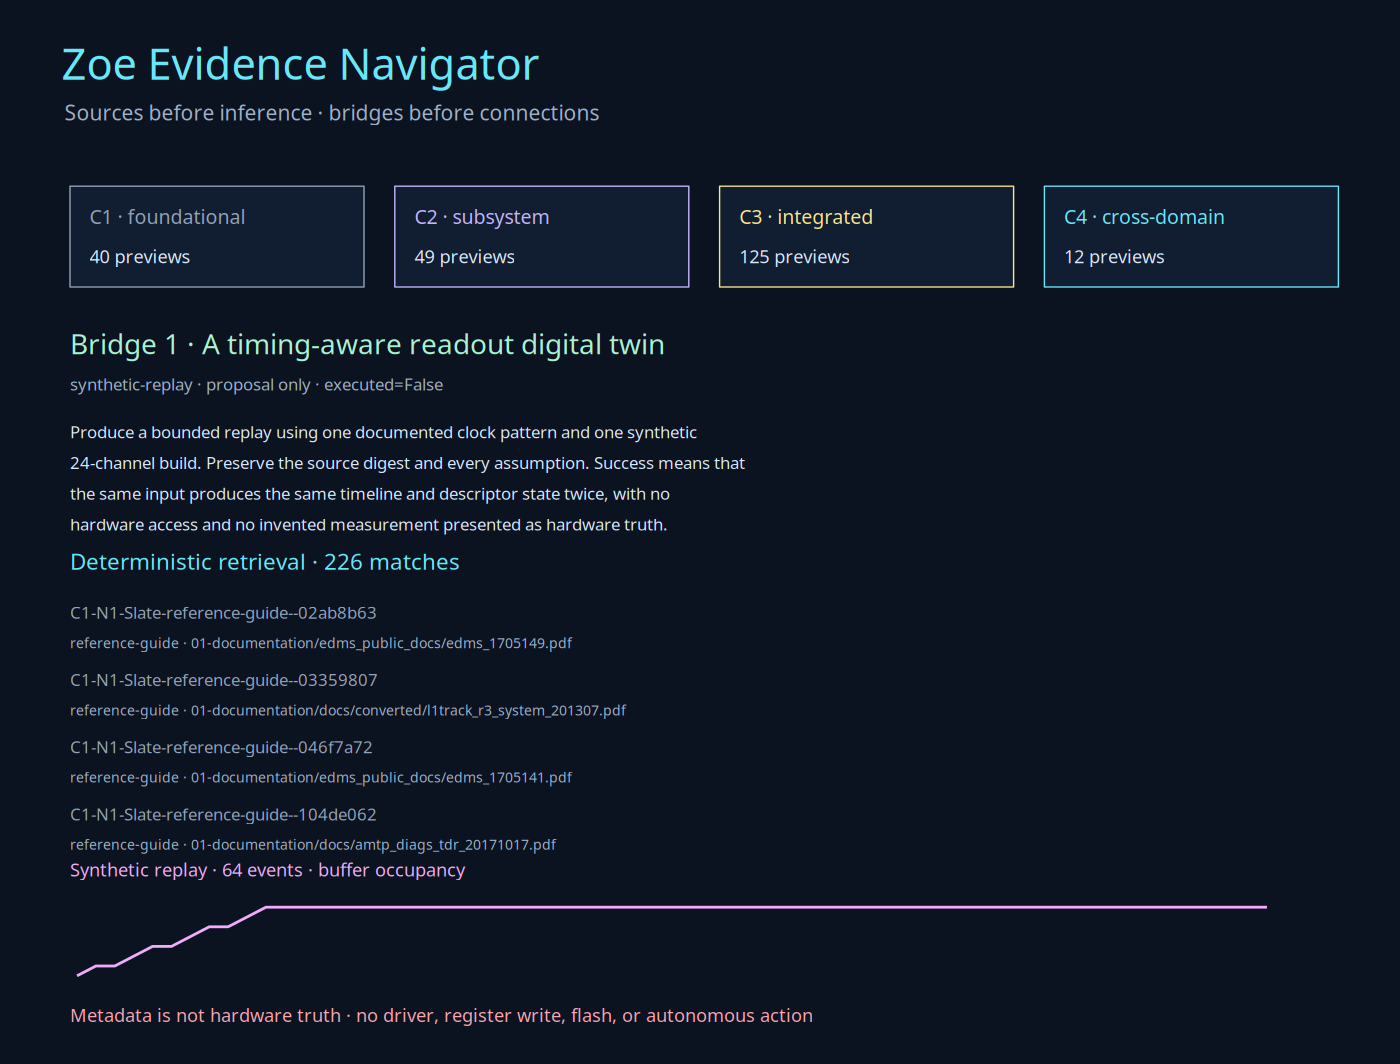
\includegraphics[width=\textwidth]{zoe-evidence.png}
\caption{Zoe Evidence Navigator: cited retrieval, source verification, bounded replay, and guarded observation. Source previews do not become live detector health.}
\label{fig:zoe-evidence-navigator}
\end{figure}

\subsection{Waveform replay and corroboration limits}
Waveform Replay reads bounded VCD, JSONL, and optional legacy WDB windows while preserving declarations, retained events, timestamps, truncation, source hashes, and normalized-document digests \cite{zoewaveformguide}. Replay is not acquisition. For clock corroboration, the classifier examines the initial payload and the first 32 subsequent equal intervals and alternating transitions. A complete sampled signature may be corroborated, ambiguous when candidates share a period or initial state, or unmapped. Matching a period alone is insufficient, and even a unique sampled period does not prove identity outside the retained window.

The cited external CERN mapper processed 10,759,544 events across 363 storage streams and reported one corroborated clock, two ambiguous streams, and 360 unmapped streams. Zoe does not rerun that large analysis or bundle its raw waveform corpus. Its independently tested preview uses four synthetic traces and preserves duplicate-signature ambiguity.

\begin{figure}[htbp]
\centering
\begin{tabular}{@{}c@{}c@{}}
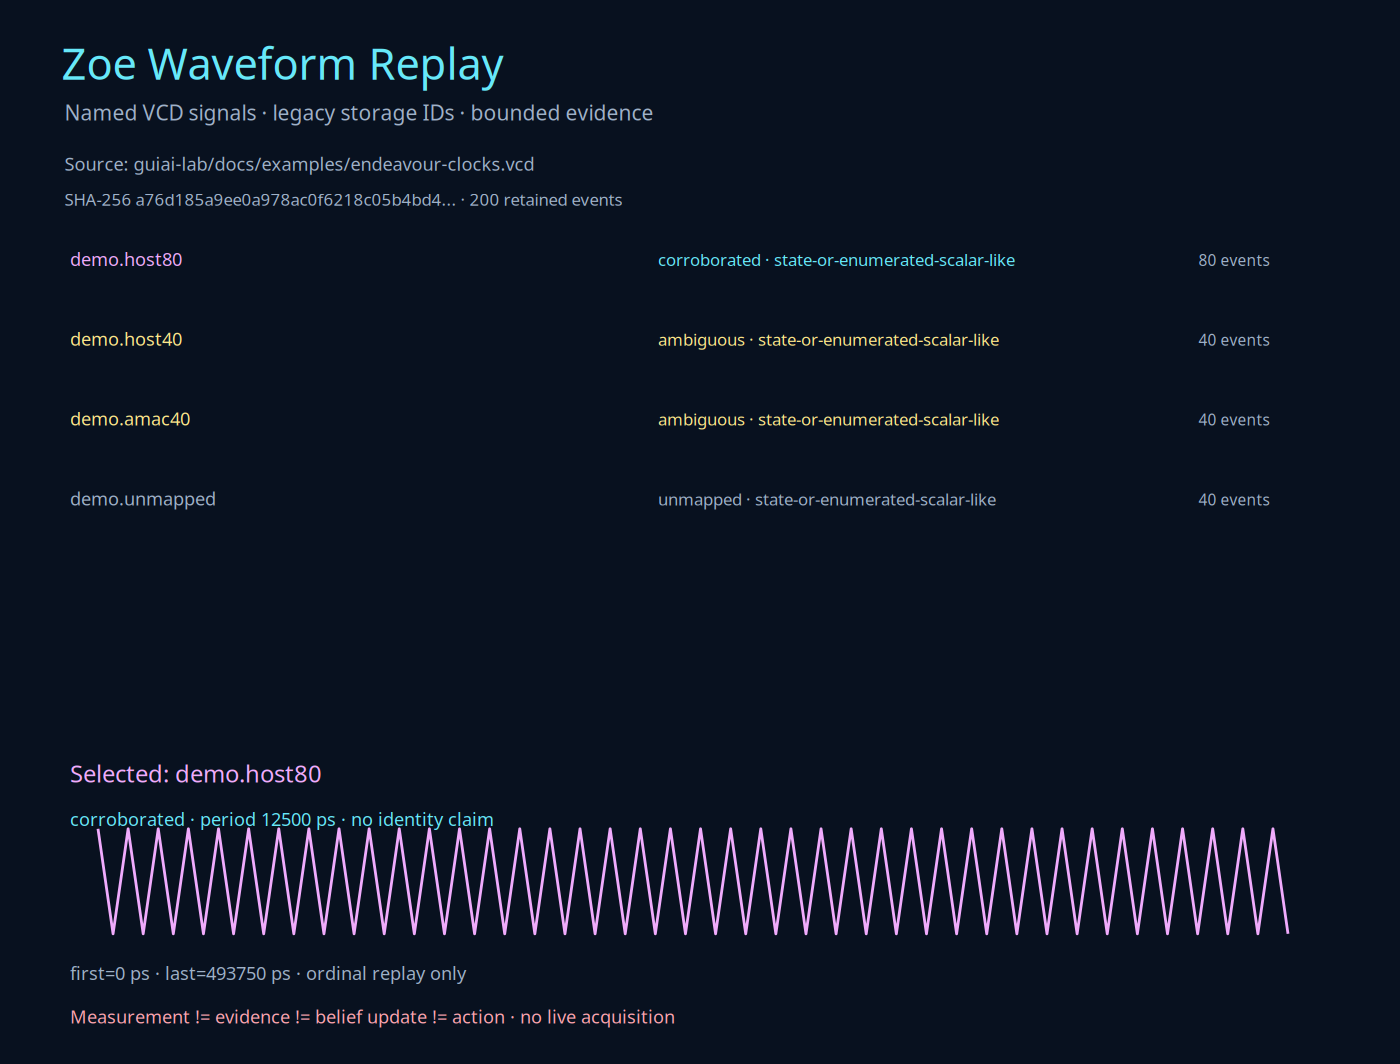
\includegraphics[width=0.48\textwidth]{zoe-waveform.png}&
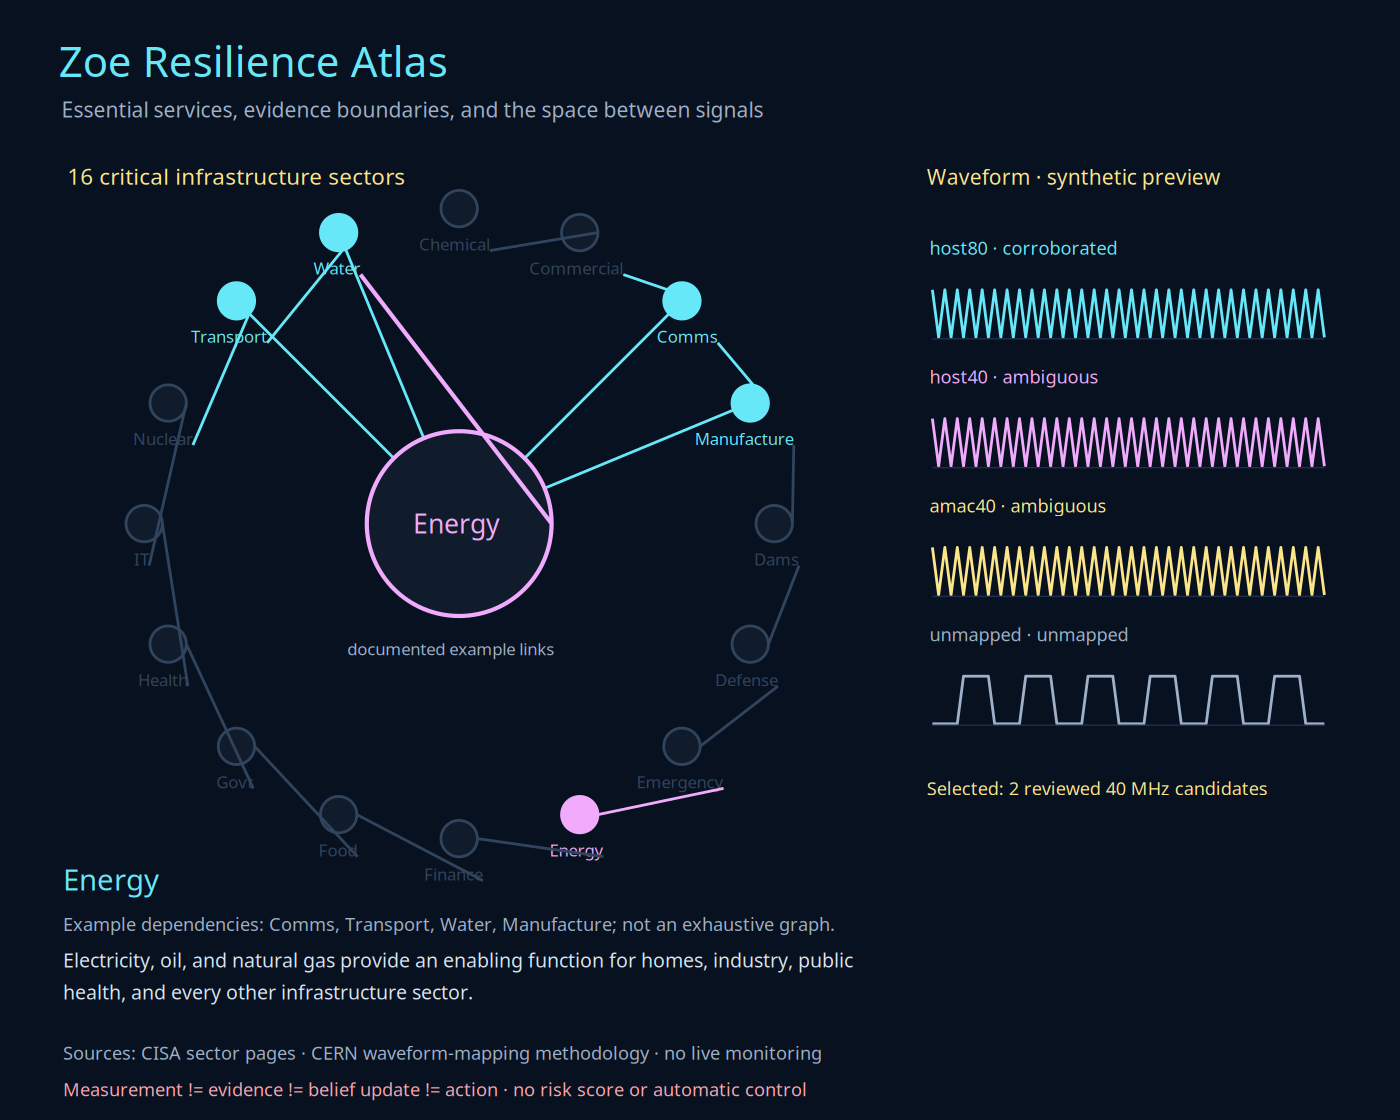
\includegraphics[width=0.48\textwidth]{zoe-resilience.png}
\end{tabular}
\caption{Waveform Replay and the Resilience Atlas preserve evidence limits. Neither performs live acquisition, infrastructure monitoring, risk scoring, or hardware control.}
\label{fig:waveform-resilience}
\end{figure}

The Resilience Atlas combines original summaries of the 16 US critical-infrastructure sectors with this small signature laboratory. Dependency links are selected public examples, not causal or exhaustive models. It contacts neither CISA nor CERN and assigns no sector risk score.

FELIX observations describe source artifacts rather than connected hardware or live detector health. The Protocol Lab preserves recovered SPECS serial-framing and AMAC reply examples with checksum and long-read boundaries; its displayed records are model and recorded examples, not new proof of correctness or permission to issue device commands.

\begin{figure}[htbp]
\centering
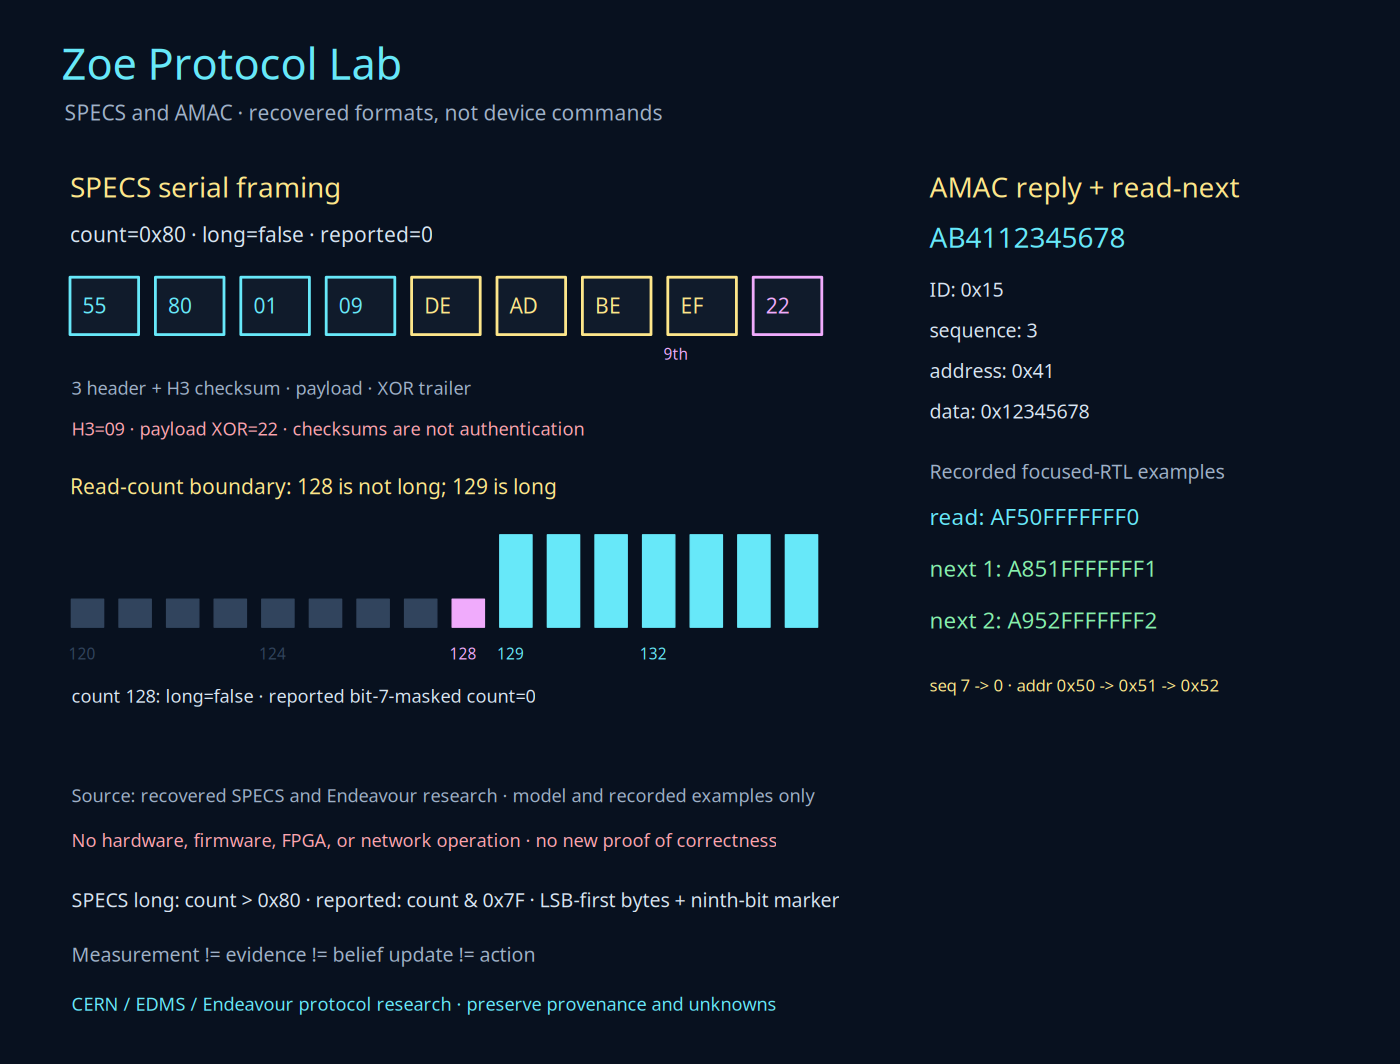
\includegraphics[width=\textwidth]{protocol.png}
\caption{Zoe Protocol Lab: recovered SPECS and AMAC protocol examples. No hardware, firmware, FPGA, or network operation is performed, and checksums are not authentication.}
\label{fig:protocol-lab}
\end{figure}

Patchbay separately inspects firmware formats and signs new update capsules. Its acceptance condition requires
\begin{equation}
\text{authenticity established}=
\text{signature valid}\;\land\;\text{artifact match}\;\land\;\text{trusted-key match}.
\label{eq:patchbay-authenticity}
\end{equation}
A self-contained public key alone is not publisher trust. Acceptance commands require an explicit execution flag and declared writes require a separate hardware-write flag. No physical hardware operation was executed for the paper integration.

\begin{figure}[htbp]
\centering
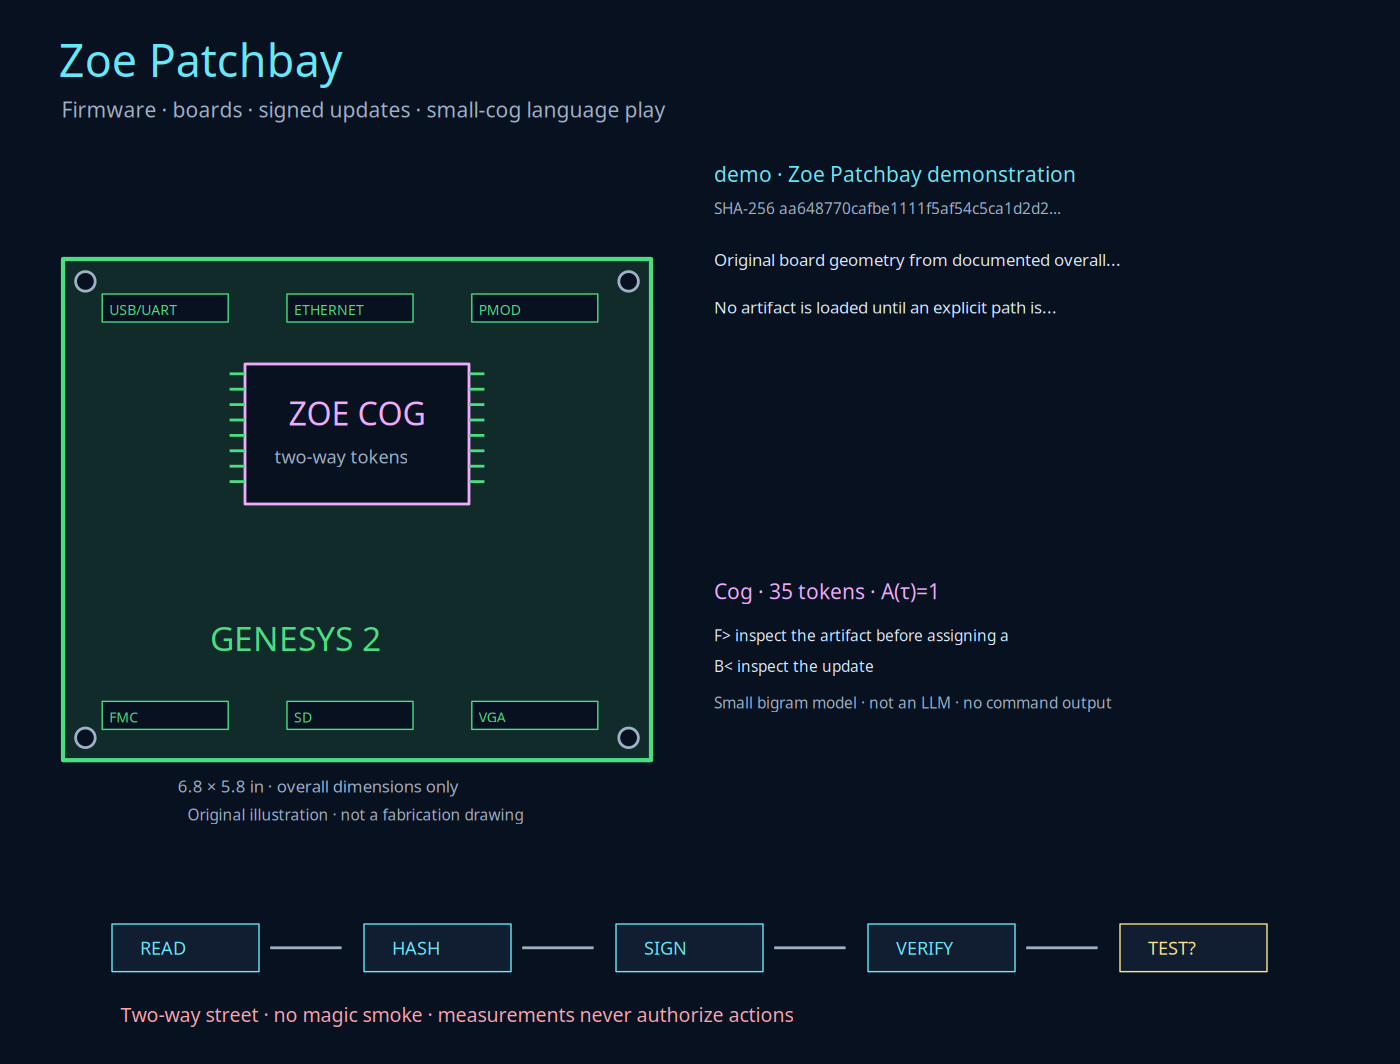
\includegraphics[width=\textwidth]{patchbay.png}
\caption{Zoe Patchbay: firmware inspection, hashing, signing, verification, and explicit acceptance boundaries. The board illustration is not a fabrication drawing and Cog output is not a command channel.}
\label{fig:patchbay}
\end{figure}

\section{Scoped verification and later audit}
The original Zoe proof of concept recorded the matrix in Table~\ref{tab:zoe-verification}. These are historical, component-scoped software results, not independent scientific replication.
\begin{table}[htbp]
\centering
\caption{Verification matrix preserved from the original Zoe proof of concept.}
\label{tab:zoe-verification}
{\scriptsize
\begin{tabularx}{\textwidth}{p{3.7cm}p{3.3cm}X}
\toprule
Area&Recorded result&Scope\\
\midrule
Zoe native&25 passed&X11 observation, notebook, host launch, Allen atlas, research, and export workflows\\
Zoe headless&21 passed, 4 native-only skips&Core, Allen atlas, memory, CLI, and evidence behavior without display\\
brain-gem headless&13 passed, 3 native-only skips&Standalone notebook, chambers, memory, and CLI\\
Broader GEM native&20 passed&Constraints, VDI, replay, dragging, and exports\\
Accessible Q-Volume&Toy arithmetic passed&Strict equality, filtrations, $-1$/$+3$ changes, and two-way JSON\\
Research conformance&17 passed&Strict volume, Procrustes, toy continuations, rhythm evidence, and Bayesian updates\\
Original model cases&16 verified&Saved distributions, ranks, counts, entropy, and hashes\\
BioBERT&120 cases, 54 candidates&Independent metrics and split recomputation\\
Cerotto&64 normal and 64 sanitizer passed&One EWF-dependent skip per suite\\
PALA&25 Rust tests, 125 integration checks&Two optional skips; recovery and format behavior\\
Interactive browser&23 particles, zero external requests/errors&Desktop, mobile, reduced motion, and controls\\
Packaging&Wheel and source distributions passed&Installed notebook, HELEN asset, conformance, and export checks\\
\bottomrule
\end{tabularx}}
\end{table}

A later November 7 audit of Zoe revision \texttt{8fcdcfe4} directly exercised both accessible-volume implementations, verified the strict comparison and threshold equality exclusion, rehashed and reloaded the 23-event knowledge chain, and recomputed all sixteen comparison and 120 BioBERT cases without fresh inference. A focused integration run completed 24 tests: 23 passed and one native-only test skipped. An isolated native unified test then failed because \texttt{UnifiedNativeCase} still expected eleven links after recording a Kevlar source while the implementation intentionally recorded both the observation and its declared Zoe link, producing twelve. The stale assertion remained an open engineering follow-up in that audit.

The audit also noted the absence of a root integrated CI workflow, a comparison verifier that rewrites tracked summaries and timestamps, two documentation inconsistencies, and the lack of a tagged PDF structure tree. Earlier all-pass records are not substituted for these later observations. The audit was not an exhaustive security review, fresh model benchmark, hardware validation, or certification of deployed behavior. This monograph preserves both the positive checks and the unresolved engineering findings.

\section{From review-gated Zoe to an executable internal loop}
The original proof of concept explicitly disclaimed autonomous decision-making. Its measured agency stopped at proposals and recommendations. The next part describes a separate extension that adds goal authorship, value-based selection, and guarded in-memory execution. The extension does not retrospectively change the evidence status of every Zoe component: most modules remain review-gated, external actuation remains prohibited, and the full-autonomy predicate applies only to the newly implemented loop.
